\documentclass[../Main.tex]{subfiles}
\begin{document}

\section{Comparison of Existing Alternative Games}
\label{chap:comparison_of_existing}
To more compare the alternative aspects of all the games mentioned in this chapter, the model based on the categories of characteristics presented in Chapter \ref{chap:what_is_alternative} has been used. It gives a quick overview of how the game differs and presents concrete characteristics for all the games in each of the six categories. The model in Table \ref{tab:existing_games} is a simplified version of the complete model found in Appendix \ref{appendix:complete_model}. The rows not used have been omitted for readability. A complete version can be found in Appendix \ref{appendix:complete_model}. 

\begin{table}[H]
    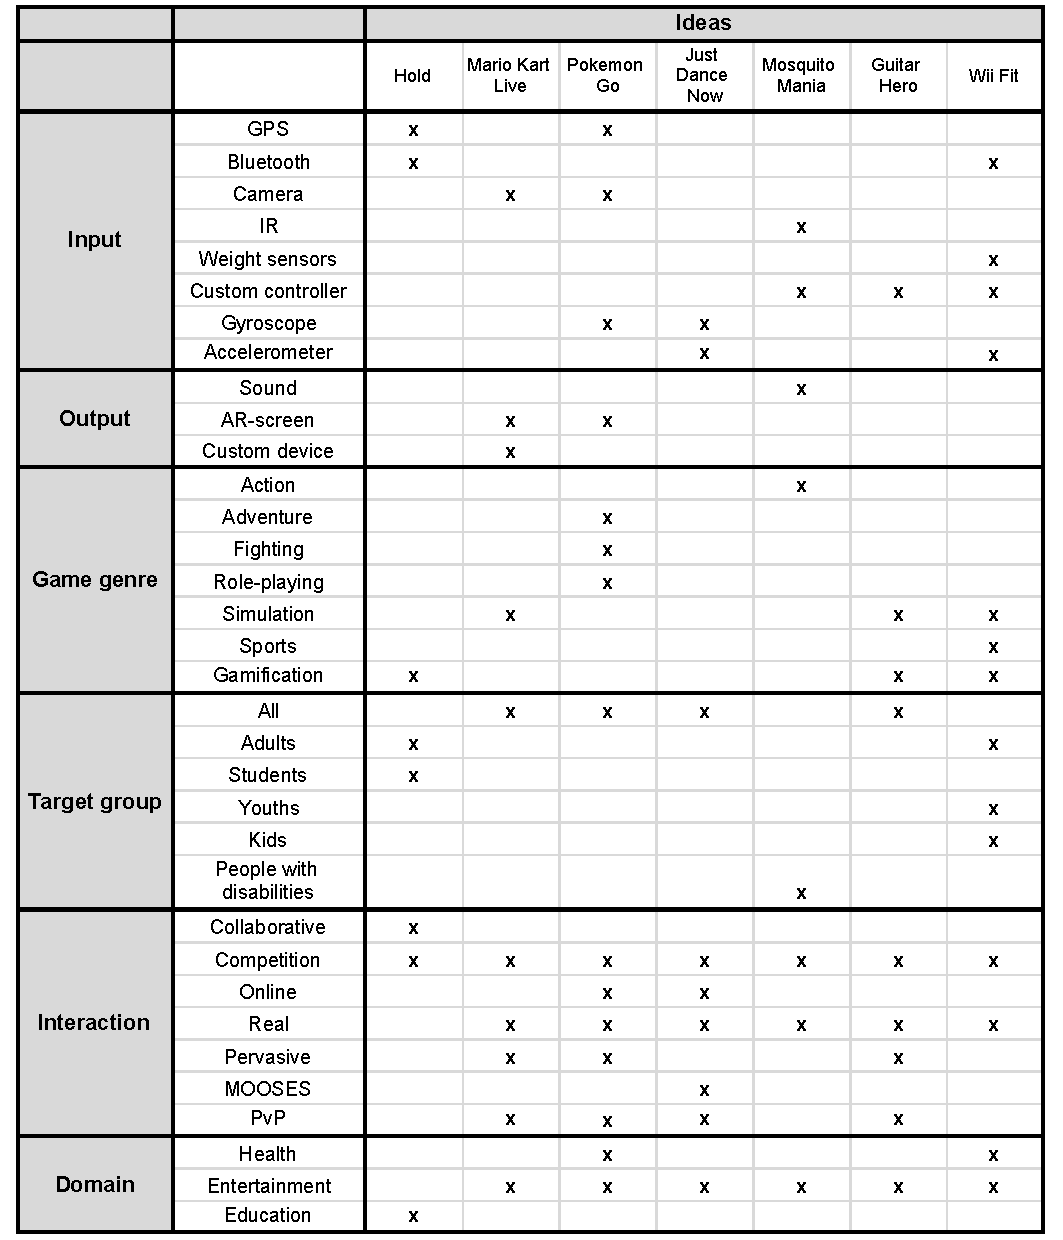
\includegraphics[width=1\textwidth]{Images/Models/ExistingGames.pdf}
    \caption{Existing alternative games characteristics}
    \label{tab:existing_games}
\end{table}

\subsection{Analysis of Input}
The first section of the model shows a wide range of \textit{input} types used in the games. The variation of input types is likely to come from the platform in use. Most mobile phones used today include various input sensors that can be used to develop alternative game concepts. GPS, Bluetooth, gyroscope are examples of such sensors.

The games Hold, Pokémon Go, and Just Dance Now are totally or partially developed for mobile platforms. Hold and Pokémon Go uses the device’s GPS to use the context of the player’s location in the game. The location-aware feature creates a better in-game experience, and players are forced to move to unlock certain features. Pokémon Go and Just Dance Now both take advantage of the phone’s gyroscope. The gyroscope can detect rotation, and for these games, the rotation tells the game how the mobile device is positioned in the real world. Just Dance Now also uses the accelerometer to track the player’s movement while dancing. The use of both gyroscope and accelerometer determines if the player is hitting the right moves at the right time, which gives better accuracy and better player-experience in this alternative game.

Guitar Hero, Wii Fit, and Mosquito Mania all use custom controllers. In the early days of games, many games used to have custom controllers \citep{overmars_brief_2012}. However, this was not fortunate for the user because it forced them to buy new controllers for each game. Nowadays, custom controllers are rare because games are often produced for specific consoles that already have an official controller. Furthermore, non-custom controllers can cause a poor user experience because they might not have an optimal or logical design. The Guitar Hero, Wii Fit, and Mosquito Mania are examples of games not suited for the standard console controller. In these games, it makes sense to use a custom controller more fit for the game's purpose. An unusual controller used as input is a classic example of an alternative game.


\subsection{Analysis of Output}
The second section of the model looks at the alternative use of \textit{output} in games. Even though today’s games often use sound effects and music, this does not make them alternative. Mosquito Mania uses sound in a more alternative scenario, as this is the only output in the game. The game focuses on the player's ability to sense the sound's direction, which is an alternative way of challenging the player's hearing instead of the eyesight.

Furthermore, Pokémon Go and Mario Kart Live use the camera as an input to produce an Augmented Reality (AR) output. AR technology is alternative in games because projecting artificial objects onto the real world is based on interpreted input. In both games, players use a handheld device. AR in mobile devices is available for the consumer considering the technology within the device. However, mobile devices do not create an immersive gaming experience compared to an AR headset.


\subsection{Analysis of Game Genre}
A selection of \textit{game genres} is listed in the third section of the table. These game genres themself do not make games alternative. However, they do tell something about what type of game it is. There is one exception to this: gamification. Gamification is alternative because it gamifies activities and tasks to make it fun and engaging while motivating the player. Hold, Guitar Hero, and Wii Fit are all gamification of activities or issues. Hold gamifies and rewards players for putting the phone down, Guitar Hero gamifies playing the guitar, and Wii Fit gamifies and motivates working out. Furthermore, games can also be classified within multiple genres, making the game more alternative. However, this is not implied.

\subsection{Analysis of Target Group}
The identified \textit{target groups} can be found in the fourth section of Table \ref{tab:existing_games}. All games have one or more dedicated target groups, corresponding to everyone or a distinguished set of users. The target groups might overlap or intersect; for instance, students and young adults intersect. Mario Kart Live, Just Dance Now, and Guitar Hero are some of the games that can be played by most people. These games might, however, address a younger crowd. Mosquito Mania is a game that can be played by most people, however, as an audio game the game can also be played by people with visual impairment.

\subsection{Analysis of Interaction}
The fifth section of the table displays the types of \textit{interactions} that have been identified in the existing games studied in Chapter \ref{chap:existing_games}. Interaction types can be found in all ordinary games and do not imply that a game is alternative. However, the type of interaction can be alternative in how player interaction is accomplished. All of the seven games use a combination of interaction methods, and all games include some degree of interaction through competition. Competition can be accomplished in numerous ways in real-time or by a scoreboard. Just Dance Now offers, like many other games, different player modes. Players can compete online in real-time, PvP, multimodal, or get high scores for the global scoreboard. These gameplay variations make the game very flexible, and players can play in whatever way they want. The other games offer similar but not so extensive features as Just Dance Now. Mario Kart Live, Pokémon Go, and Guitar Hero all include the competitive feature of PvP interaction. In these games, players communicate in the real world, but the gameplay happens in the virtual world.

Hold is the only game that includes a collaborative mode. Players can connect their device with their friends’ to boost points; if one player quits, the player will not only lose his or her focus but also stop the boosting for the collaborating players. This interaction feature is likely to strengthen the player’s motivation for not using their phones.
 

\subsection{Analysis of Domain}
The sixth and last section of the model displays the \textit{domain} of the games. Traditionally speaking, games often belong to the domain of entertainment. Some alternative games have an alternative area of use and therefore touches within one or more domains. The exercise game Wii Fit is directly connected to the domain of physical health. Pokémon Go also exploits the benefits of physical health from having players move around. The exploiting of other domains than entertainment makes these games more alternative. On the other hand, Hold is not like traditional games and does not classify under the entertainment domain. Its target group is students and is therefore used indirectly in the domain of education.

\subsection{Summary}
This chapter has focused on showcasing multiple different and typical examples of alternative games (based on our definition presented in Chapter \ref{chap:what_is_alternative}). The examples have been shortly described and compared with each other to highlight their differences. A table with the characteristics of each game has been presented and analyzed. The next chapter will shift the focus from the concept of alternative games to the technical aspect of the field. 

\biblio % Needed for referencing to working when compiling individual subfiles - Do not remove
\end{document}